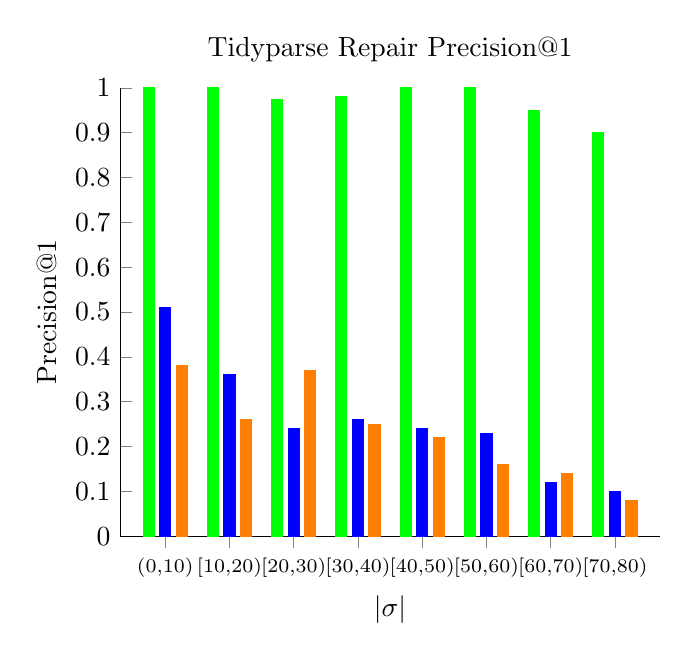
\begin{tikzpicture}
  \begin{axis}[
    xlabel={$|\sigma|$},
    ylabel={Precision@1},
    title={Tidyparse Repair Precision@1},
    ybar,
    axis lines*=left,
    xtick={0, 10, 20, 30, 40, 50, 60, 70},
    ytick={0, 0.1, 0.2, 0.3, 0.4, 0.5, 0.6, 0.7, 0.8, 0.9, 1.0},
    xticklabels={{(}0{,}10{)}, {[}10{,}20{)}, {[}20{,}30{)}, {[}30{,}40{)}, {[}40{,}50{)}, {[}50{,}60{)}, {[}60{,}70{)}, {[}70{,}80{)}},
    x tick label style={font=\scriptsize},
    ymax=1.0,
    ymin=0.0,
    bar width=4pt,
  ]

  \addplot[green, fill=green] coordinates { (0, 1.0) (10, 1.0) (20, 0.975) (30, 0.98) (40, 1.0) (50, 1.0) (60, 0.95) (70, 0.9) };
  \addplot[blue, fill=blue] coordinates { (0, 0.51) (10, 0.36) (20, 0.24) (30, 0.26) (40, 0.24) (50, 0.23) (60, 0.12) (70, 0.1) };
  \addplot[orange, fill=orange] coordinates { (0, 0.38) (10, 0.26) (20, 0.37) (30, 0.25) (40, 0.22) (50, 0.16) (60, 0.14) (70, 0.08) };

%  \legend{Δ=1,Δ=2,Δ=3}
  \end{axis}
\end{tikzpicture}